\chapter{Introduction}
\label{chpt:introduction}

This is a dissertation template. Here is the introduction text. As with this chapter, add other chapters to the dissertation and cite them in the ``main.tex'' file.


\section{Example Section}
\label{sec:examplesec1}

This dissertation template combines the work of our fore-academics to build a format that works for all of those who use \LaTeX \cite{jefferson2019policing}. We sincerely hope you find it useful \cite{shannon1948mathematical}.

You can add acronyms in the text and front table! See the comments around the acronyms command for how to include them in the front table. The first time you use an acronym in the text, use the ``\textbackslash ac\{\}'' command like with this \ac{TLA} or \ac{SOA}. After you use them the first time, it'll just appear as the acronym (like this: \ac{TLA}).

\blindtext


\section{Example Tables}
\label{sec:examplesec2}

You can make a table as follows \cite{ong1997gilbert}. Use can cross-reference items by doing things like Chapter \ref{chpt:introduction}.

\blindtext

\begin{table}[ht]
    \begin{tabular}{l|l}
        \textbf{left column} & \textbf{right column} \\ \hline
        entry1 & entry2 \\
        entry3 & entry4
    \end{tabular}
    \caption{An example table with things in it. See \url{https://www.latex-tables.com/} for a relatively-easy latex table generator. Other options include \url{https://truben.no/table/old/} and \url{https://www.tablesgenerator.com/}, but you'll find others online, too! Here, we're also showing that you can create URLs that link to external websites while still being underlined. You can use ``\textbackslash url\{\}'' for shorter URLs, but they will roll over the end of the line if they're too long. In that case, it's more accessible if you use ``\textbackslash href\{\textless url\textgreater\}\{\textless text\textgreater\}'' instead because it breaks at spaces in the text.}
    \label{tab:my-table}
\end{table}

\blindtext


\section{Example Figure}
\label{sec:examplesec3}

Check out Figure \ref{fig:the_big_house}. \blindtext

\begin{figure}
    \centering
    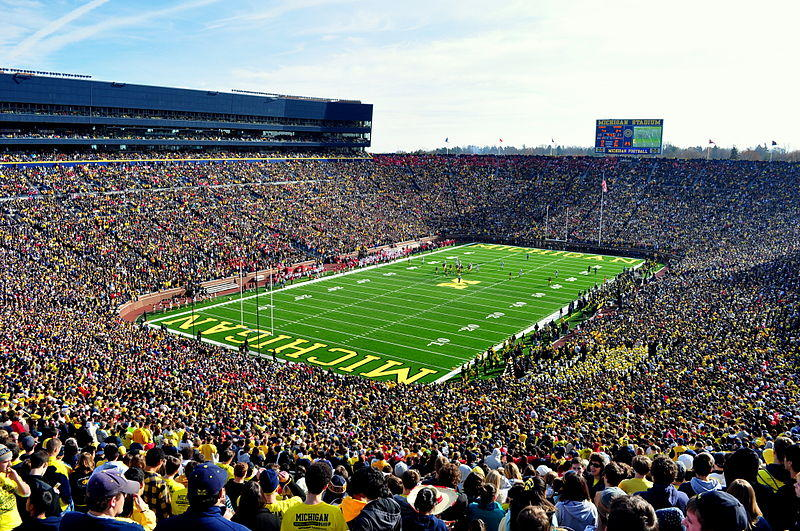
\includegraphics{chapters/figures/the_big_house.jpeg}
    \caption{The Big House, taken from Michigan Radio's article about it \cite{the_big_house}}
    \label{fig:the_big_house}
\end{figure}

\blindtext[3]